\documentclass{VUMIFPSkursinis}
\usepackage{algorithmicx}
\usepackage{algorithm}
\usepackage{algpseudocode}
\usepackage{amsfonts}
\usepackage{amsmath}
\usepackage{bm}
\usepackage{caption}
\usepackage{color}
\usepackage{float}
\usepackage{graphicx}
\usepackage{listings}
\usepackage{subfig}
\usepackage{wrapfig}
\usepackage{parcolumns}
\usepackage{enumitem}
\usepackage{array}
%PAKEISTA, tarpai tarp sąrašo elementų
\setitemize{noitemsep,topsep=0pt,parsep=0pt,partopsep=0pt}
\setenumerate{noitemsep,topsep=0pt,parsep=0pt,partopsep=0pt}
\renewcommand{\lstlistingname}{Kodo ištrauka}

% Titulinio aprašas
\university{Vilniaus universitetas}
\faculty{Matematikos ir informatikos fakultetas}
\department{Programų sistemų katedra}
\papertype{Kursinis darbas}
\title{WebAssembly panaudojamumo galimybių analizė kuriant konkurencingas naujos kartos internetines programas }
\titleineng{WebAssembly Usability Analysis in Competitive Next-Generation Web Development}
\status{3 kurso 5 grupės studentas}
\author{Kasparas Taminskas}
\supervisor{Aurimas Šimkus}
\date{Vilnius – \the\year}

% Nustatymai
%\setmainfont{Palemonas}   % Pakeisti teksto šriftą į Palemonas (turi būti įdiegtas sistemoje)
\bibliography{bibliografija}

\begin{document}
\lstset{language=C}

% PAKEISTA	
\maketitle
\cleardoublepage\pagenumbering{arabic}
\setcounter{page}{2}

%TURINYS
\tableofcontents

\sectionnonum{Anotacija}
WebAssembly technologija — sėkmingai moderniose interneto naršyklėse realizuotas naujų, atvirų žiniatinklio standartų rinkinys, suteikiantis iki šiol neregėtus greitaveikos rodiklius ir naujas programavimo galimybes žiniatinklyje. Nepaisant to, technologija kol kas išlieka tik pradiniuose vystymo etapuose, plati žiniatinklio programuotojų bendruomenė tik pradeda susipažinti su jos galimybėmis. Dėl standarto naujovės dažnai pasigirsta tam tikrų mitų ar skambių pareiškimų, tokių kaip JavaScript kalbos gyvavimo pabaiga. Šiuo rašto darbu siekiama atskleisti technologijos paskirtį, apžvelgti jos atsiradimo prielaidas ir išanalizuoti pritaikymo galimybes tose situacijose, kuriose jos atrodo prasmingos. Įgyvendinus šiuos siekius bus galima sugriauti minėtus mitus ir neteisingas spėliones.

\sectionnonum{Įvadas}
Interneto naudojimo reikšmė per 30 paskutiniųjų metų nuo žiniatinklio atsiradimo išaugo 
eksponentiškai. Nors saityno potencialas buvo pastebimas nuo pat pradžios, tačiau vargu, ar 
kas nors XX a. IX dešimtmetyje galėjo pagalvoti, jog auganti interneto reikšmė pasieks tokį 
lygį, jog tradicinės programų sistemos, turinčios didžiulę kodo bazę, kuriamos skirtingoms 
fizinėms platformoms ir programinėms aplinkoms, reikalaujančios intensyvaus mašininių resursų 
panaudojimo, bus taip pat pasiekiamos tiesiog vienu pelės paspaudimu, nepriklausys nuo 
konkrečios mašininės architektūros, programinės aplinkos ir nereikalaus jokių specialių 
diegimo etapų.

Šiomis dienomis programinės įrangos kūrimo rinkoje internetinės technologijos ir 
platformos, debesų kompiuterija yra įmonių dėmesio centre, nes galimybė pasiūlyti programinį 
produktą internetu atveria didelį konkurencinį pranašumą – klientams nebereikia įsidiegti 
programinės įrangos į savo elektroninius įrenginius, užtenka vienos programos – interneto 
naršyklės – kuri atveria plačias galimybes naudotis skirtingų tipų programomis, pateikiamomis, 
kaip paslauga klientui (angl. — Software as a Service). Be to, patys programų sistemų kūrėjai 
patiria mažesnius kaštus kurdami ir palaikydami savo produktus, nes nebelieka poreikio turėti 
skirtingų kodo bazių specifinėms operacinėms aplinkoms ar įrenginiams.

Poreikis turėti kompleksiškas programų sistemas internetinėje erdvėje kelia didelius 
reikalavimus pagrindiniams saityno technologijų kūrėjams – didiesiems naršyklių gamintojams – 
kurių technologiniai sprendimai įgalina programuotojus įgyvendinti programinius sprendimus 
internete: šios naujos kartos programos internete turi užtikrinti tokius pačius kokybinius 
reikalavimus — greitaveiką, saugumą ir patikimumą — kaip senosios. Šioje vietoje susiduriama 
su dideliais technologiniais naršyklių variklių implementacijos ir pagrindinės internetinių 
technologijų programinės kalbos – JavaScript – ribojimais, neleidžiančiais įgyvendinti 
internetinių programų visiško supanašėjimo su tradicinėmis, veikiančiomis specifinėse 
platformose. 

WebAssembly standarto specfikacija ir jos formalus įgyvendinimas naršyklių 
smėliadėžės (angl. – sandbox) aplinkose siūlo sprendimą – binarinio formato kodo vykdymą 
greitaveikai imliose programų sistemų verslo logikos vietose papildant tradicinį JavaScript 
kodą. Ši technologinė naujovė, apibrėžta Pasaulinio žiniatinklio konsorciumo (W3C) ir palaikoma
visų modernių naršyklių kūrėjų, leidžia ženkliai sumažinti likusius techninius barjerus tarp 
naujos kartos internetinių programų sistemų ir tradicinių, nuo vykdymo aplinkos priklausamų 
sprendimų, todėl atveria saityne dar neišnaudotas rinkos perspektyvas, sėkmingai gyvuojančias
tradicinėse platformose. 

\sectionnonum{Tikslas ir uždaviniai}
Šio rašto darbo tikslas – pasiūlyti konkrečius praktinius variantus, kaip standartas 
gali būti integruotas į naujus ir jau egzistuojančius internetinius programinius sprendimus. 
Šie būdai leis programų sistemų kūrėjams išnaudoti stipriąsias technologijos dalis ir taip 
įgauti didesnį konkurencinį pranašumą internetinėje programų sistemų rinkoje.

Išsikeltas darbo tikslas realizuotas įgyvendinant užsibrėžtus tarpinius uždavinius, padedančius įsigilinti į problemos esmę:
\begin{itemize}
    \item Prielaidų, paskatinusių WebAssembly technologijai atsirasti, analizė
    \item WebAssembly koncepcinės veikimo logikos suvokimas
    \item Skirtingų WebAssembly pritaikymo būdų analizė
\end{itemize}

\section{Žiniatinklio ekosistemos technologinė raida}

Siekiant geriau suprasti dabartinę padėtį, kurioje buvo pristatytas WebAssembly standartas ir kokius poreikius jis patenkina, yra būtina apžvelgti viso žiniatinklio populiarumo augimą ir jo technologinę raidą.

\subsection{Interneto populiarumo augimas}

Interneto bendruomenę sudarančių žemės gyventojų skaičius šiuo metu viršija pusę visos Žemės populiacijos. Šis augimas, prasidėjęs 1995 metais, kai Saitynas atsivėrė plačiai pasaulio bendruomenei, nestoja ir toliau, tą galima pastebėti iš \ref{fig:internet_usage} paveikslėlyje matomos viešos metinės statistikos. 

\begin{figure}[h!]
  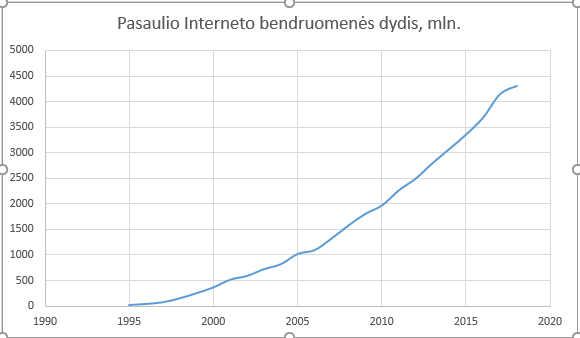
\includegraphics[scale=1]{interneto_naudojimo_statistika.png}
  \caption{Interneto bendruomenės narių skaičius 1995—2018}
  \label{fig:internet_usage}
\end{figure}

Ši statistika tik patvirtina plataus Interneto technologijų pritaikymo poreikio aktualumą ir didelę atsakomybę, tenkančią šių technologijų vedliams — interneto naršyklių kūrėjams. Žiniatinklis jau seniai nėra skirtas tik informacijos paieškai ir dalinimuisi, ką įgalino pradinės saityno technologijos — HTTP protokolas, HTML ir CSS žymėjimo kalbos. Šiuo metu vis didesnį pagreitį įgauna virtualios realybės, žaidimų industrijos, filmų ir muzikos sferų, neuroninių tinklų kūrimo ir analizės įrankiai. Deja, bet dažnai šių sprendimų pasiūlymas Internete būna ribotas dėl fundamentalių architektūrinių principų, kuriais paremtas programinio kodo vykdymas interneto naršyklėse.

\subsection{Programinio kodo vykdymas naršyklėse}
Interneto naršyklė architektūriniu požiūriu yra itin sudėtinga programa, nes procese nuo resurso parsiuntimo iš nutolusio serverio iki jo grafinio atvaizdavimo naršyklės lange dalyvauja daug sisteminių programos komponentų, nurodytų \ref{fig:browser_architecture} paveikslėlyje. 

\begin{figure}[h!]
  \begin{center}
  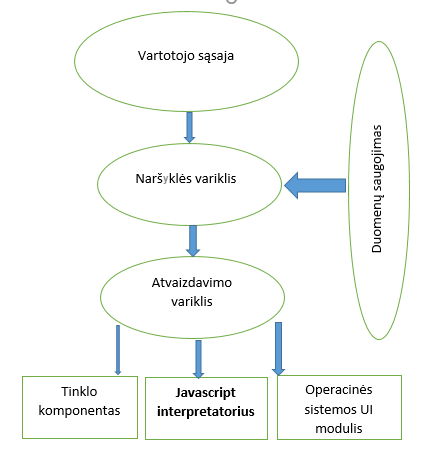
\includegraphics[scale=0.8]{naršyklės_architektūra.png}
  \end{center}
  \caption{Aukšto lygio interneto naršyklės veikimo principas}
  \label{fig:browser_architecture}
\end{figure}

Vienas esminių šios schemos komponentų — Javascript interpretatorius — žiniatinkliui suteikia dinamiškumą ir leidžia vykdyti skriptus, parašytus Javascript programavimo kalba, tiesiog naršyklėje. Interpretatoriaus rezultatai siunčiami atvaizdavimo varikliui, kuris pasirūpina jų išdėstymu interneto aplikacijoje. Norint geriau suprasti Javascript vykdymo greitaveikos problemas, būtina apžvelgti du fundamentaliai skirtingus programinio kodo transliavimo į mašininį kodą principus.

\subsubsection{Transliavimo metodai}
Programinės kalbos dažniausiai skirstomos į statines ir dinamines, t.y. ar programiniai tipai egzistuoja kompiliavimo metu, ar yra nustatomi kodo vykdymo metu (angl. — at runtime). Keletas šioms skirtingoms šeimoms priklausančių kalbų:
\begin{enumerate}
    \item Statinės: C, C++
    \item Dinaminės: Python, Rust, Javascript
    \item Turinčios abiejų šeimų požymių: Java, C\#
\end{enumerate}

Pagal tai, kuriai šeimai kalba priklauso, skiriasi būdas, kuriuo išeities kodas yra verčiamas į mašinines tam tikros architektūros procesoriaus instrukcijas.

\subsubsubsection{Kompiliavimas ir interpretavimas}
\ref{tab:kompiliavimas_interpretavimas} Lentelėje pateikti šių transliavimo metodų skirtumai ir ypatumai, atskleidžiantys konkretaus metodo privalumus ir trūkumus tam tikrose situacijose. Būtina pažymėti, kad universalaus sprendimo, kuris variantas geresnis nėra, todėl programavimo pasaulyje derinami abu variantai.

\begin{table}[H]
  \centering
  \caption{kompiliavimo ir interpretavimo skirtumai}
  {\begin{tabular}{|m{13em}|m{13em}|} \hline
     Kompiliavimo savybės & Interpretavimo savybės \\
    \hline
    Transliuojamas visas išeities kodas iš karto & Kodas transliuojamas dalimis 
 sakinys po sakinio \\
 \hline
     Pradinis kodo analizės etapas daug greitesnis, 
     tačiau vykdymo greitaveika lėtesnė  & Pradinė kodo analizė 
     užima proporcingai didesnę laiko dalį, nei interpretavimo atveju, 
     tačiau vykdymas ženkliai greitesnis  \\
    \hline
     Generuojamas tarpinis objektinis kodas, kuris
 reikalauja surišimo žingsnio, papildomai naudojama atmintis & Nėra generuojama jokio tarpinio kodo \\
 \hline
 Programa transliuojama iki pirmos klaidos, kuomet 
 vykdymas stabdomas, todėl programos derinimas lengvas & Klaidos pranešimas 
 generuojamas tik atlikus pilną kodo analizę, derinimo žingsnis daug sunkesnis \\
 \hline
  \end{tabular}}
  \label{tab:kompiliavimas_interpretavimas}
\end{table}

\subsubsection{JavaScript kalbos savybės}

Nuo pat žiniatinklio atsiradimo pradžios interneto technologijų branduolį sudaro Javascript programavimo kalba, kurios prototipas per 10 dienų buvo sukurtas 1995 metais kompanijos Netscape Communications. Ši programavimo kalba žiniatinklyje iki šiol užėmė visišką monopoliją, interneto aplikacijų klientinės dalies kūrimas be jos yra tiesiog sunkiai įsivaizduojamas atvejis. Kalbos populiarumą ir išplitimą patvirtina GitHub saugyklos repozitorijų statistiniai duomenys, pagal kuriuos kalba jau ilgą laiką pirmauja turėdama virš 320000 aktyvių repozitorijų. 

\subsubsubsection{Dinaminė prigimtis}

Javascript programavimo kalba pasižymi dinaminiais tipais, t.y. kintamieji savo reikšmių tipus gali keisti skripto vykdymo metu. Žemiau pateikta kodo ištrauka yra visiškai validi ir leidžiama interpretatoriaus.

\begin{center}
\begin{small}
\begin{verbatim}
var x = 10;                   //console.log(x) => 10
x = "sveiki";                 //console.log(x) => sveiki
x = {                         //console.log(x) => [Object]
    a: "sveiki is objekto",
    b: 10,
    c: true
}
\end{verbatim}
\end{small}
\end{center}

Ši kalbos savybė programuotojams užtikrina lanksčias galimybes greitai ir ekspresyviai rašyti programinį kodą, kurio vykdymo pradžia yra itin greita, nes Javascript yra interpretuojama kalba. Deja, bet ši kalbos dinamiškumo savybė itin trukdo vykdyti programinį kodą, kuris imlus operacijų kiekiui, reikalauja didelės greitaveikos, nes interpretatorius privalo kiekvieną kartą tikrinti, ar vykdomas kodas turi tuos pačius tipus 

\subsubsection{Naršyklių gamintojų greitaveikos problemos sprendimas}

Didieji naršyklių gamintojai siekdami išnaudoti geriausias interpretatorių ir kompiliatorių savybes įdiegė naujus papildomus žingsnius Javascript kodo vykdymo variklyje procese. Dauguma Javascript variklių šiuo metu naudoja labai panašios architektūros kodo kompiliavimo procesus, todėl panagrinėsime vieno jų — Google kompanijos kuriamo ir palaikomo atviro kodo variklio — veikimo principus.

\subsubsubsection{V8 variklio Javascript kodo vykdymo etapai}
Iki 2008 metų Javascript kodo vykdymas naršyklėse buvo pastibimai lėtesnis, tačiau prasidėjus naršyklių gamintojų „greitaveikos karams" buvo įdiegti JIT (angl. — Just in Time) kompiliatoriai, kurie pastebimai padidino greitaveikos rodiklius. Šių kompiliatorių vietą Javascript kodo vykdymo grandinėje galima matyti \ref{fig:v8_pipeline} paveikslėlyje.

\begin{figure}[h!]
  \begin{center}
  \includegraphics[scale=0.8]{V8_kompiliavimo_grandinė.png}
  \end{center}
  \caption{Chrome naršyklėje naudojamo V8 Javascript variklio kodo vykdymo grandinė}
  \label{fig:v8_pipeline}
\end{figure}

\section{WebAssembly standarto specifikacija}

WebAssembly yra standartų rinkinys, sukurtas ir palaikomas Pasaulio žiniatinklio konsorciumo (angl. — World Wide Web Consorcium), apibrėžiantis koncepcinį žemo lygio mašinio kodo formatą, į kurį gali būti verčiamos aukšto lygio programavimo kalbos.

\subsection{Programavimo kalbos ypatybės}
WebAssembly yra žemo lygio, statinė programavimo kalba, turinti vos keletą kintamųjų tipų:

\begin{itemize}
    \item Sveikojo skaičiaus: i32, i64
    \item Slankaus kablelio: f32, f64
\end{itemize}

Lyginant šią kalbą su JavaScript, kuri yra dinaminė, aukšto lygio, galima pastebėti, jog nėra tokios įvairovės ir lankstumo — jokių eilučių tipų, masyvų, objektų. Funkcijų parametrų ir grįžimo reikšmės privalo būti griežtai deklaruotos ir apribrėžtos. Taip pat WebAssembly specifikacijoje apibrėžti statiniai užvardinti funkcijų importavimai ir eksportavimai.


\subsection{Koncepcinio mašininio kodo vykdymas}
WebAssembly mašininis kodas skirtas vykdyti steko pagrindu veikiančioms virtualioms mašinoms. Virtuali mašina yra aukšto lygio abstrakcijos sluoksnis, leidžiantis programinį kodą vykdyti skirtingose operacinėse sistemose ir fizinėse architektūrose, todėl WebAssembly mašininį kodą lyginti su tradiciniu konkrečios fizinės architektūros mašininiu kodu būtų neteisinga. Supaprastinta WebAssembly programinio kodo vertimo į konkrečią fizinę architekūrą schema pateikta \ref{fig:wasm_compilation} paveikslėlyje. Programinės kalbos dažnai turi tarpines kodo išraiškas (angl. — Intermediate Representation), skirtas programinį kodą versti į konkrečios fizinės architektūros mašinininį kodą. WebAssembly mašininis kodas sugeba priimti šį tarpinį formatą, naršyklių implementacijos sugeba atlikti Wasm kodo transliavimą į konkrečią fizinę architektūrą be sudėtingų ir laikui imlių žingsnių. 

\begin{figure}[h!]
  \begin{center}
  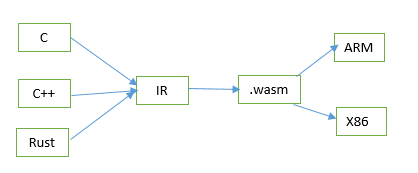
\includegraphics[scale=0.8]{webassembly_kompiliavimas.png}
  \end{center}
  \caption{.wasm kodo kompiliavimas}
  \label{fig:wasm_compilation}
\end{figure}

\subsection{Virtualios mašinos implementacija}

WebAssembly formatas sukurtas steko pagrindu veikiančiai mašinai — tai specialus virtualios mašinos implementacijos atvejis, kai aritmetiniai ir loginiai operandai ir operacijų rezultatai saugomi steko pagrindo duomenų struktūroje, o išėmimo ir įdėjimo tvarka grįsta LIFO (angl. — Last—in First—out) principu. 

\begin{figure}[h!]
  \begin{center}
  \includegraphics[scale=0.62]{sudėtis_steke.png}
  \end{center}
  \caption{Sudėtis steke}
  \label{fig:stack_addition}
\end{figure}

Šis virtualios mašinos implementacijos būdas užtikrina efektyvią greitaveiką, nes nereikia išreikštinai žinoti operandų atminties adresų — naudojama steko viršūnės rodyklė (angl. — Stack Pointer), o kiekiena įdėjimo/išėjimo operacija pakeičia šios rodyklės reikšmę vienetu.
Kaip matome \ref{fig:stack_addition} paveikslėlyje, paprastai sudėties operacijai steko implementacijos atveju reikia keturių komandų. Egzistuoja registrais grįsta virtualio mašinos realizacija, kurioje sudėtis gali būti išreiškiama viena operacija, tačiau tokiu atveju reikia nurodyti ir žinoti registrų adresus. Neteisinga teigti, jog viena implementacija universaliu atveju geresnė už kitą, efektyvumą lemia naudojimo kontekstas.

\section{WebAssembly panaudojamumo būdai}
Standarto panaudojimo galimybes kuriant interneto programas galima skirstyti pagal pritaikymo skalę — kokį proporcinį visos programos kiekio dalį užima WebAssembly kodo bazė.

\subsection{Modulio integracija į egzistuojantį JavaScript projektą}
Dar iki WebAssembly standarto atsiradimo, nuo ECMAScript2015 standarto specifikacijos išleidimo, JavaScript ekosistema tapo daug moduliaresnė, nei buvo prieš tai. Ši technologinė savybė leidžia enkapsuliuoti realizacijos logiką, o klientui pateikti tik ribotą programinę sąsają (angl. — Application Programming Interface), skirtą naudotis paketu ar moduliu. WebAssembly standartas kuriamas atsižvelgiant į modulių naudą ir poreikį.

\subsubsection{Problemos apibrėžimas}
Sakykime, jog turime realizavę internetinę programą, kurios esminė verslo logikos dalis atlieka procesoriaus ar vaizdo plokštės darbo laikui imlias operacijas. Mūsų klientai džiaugiasi, jog esame pirmieji realizavę tokio tipo sistemą internete, tačiau skundžiasi, jog darbas su sistema nėra sklandus, juntamas dažnas uždelsimas. Tokių sistemų pavyzdžiai galėtų būti vaizdo, garso kodavimo ir apdorojimo programos, papildytos realybės (angl. — Augmented Reality) sprendimai, dirbtinio intelekto sistemos. 
\subsubsection{Sprendimas}
Galima bandyti susidariusią problemą spręsti pertvarkant egzistuojantį centrinį verslo logikos algoritmą, parašytą JavaScript programavimo kalba ir stebint greitaveikos rodiklius, tačiau anksčiau ar vėliau neabejotinai bus pasiekta riba, kurios peržengti su esama technologija nebus įmanoma, nes pati kalba nesuteikia prieigos prie žemų programinių konstruktų, tokių kaip savarankiškas ir efektyvus atminties išskyrimas ir valdymas. 
\subsubsubsection{WebAssembly integracija}
Šioje vietoje atsiranda galimybė panaudoti enkapsuliuotą WebAssembly modulį, kuris savyje turėtų realizuotą centrinį skaičiavimų logikos algoritmą. Jeigu mūsų internetinės programų sistemos sprendimas kilo iš jau anksčiau egzistavusios darbalaukinės programos, didelė galimybė, jog mums net nereikės perrašinėti jokios verslo logikos kita kalba. Sakykime, jog savo algoritmą rašome C kalba, imituokime mūsų verslo logikos algoritmą realizuodami Burbulo metodo (angl. — Bubble Sort) rikiavimo funkciją:

\begin{center}
\begin{small}
\begin{verbatim}
int8_t* EMSCRIPTEN_KEEPALIVE bubbleSort(int8_t *buf, int n) {
    for (int i=0; i<n—1;i++) {
        for (int j=0;j<n—i—1;j++) {
            if (buf[j]>buf[j+1]) {
                swap(&buf[j], &buf[j+1]);
            }
        }
    }
    return buf;
}
\end{verbatim}
\end{small}
\end{center}

Verta paminėti, jog EMSCRIPTEN\_KEEPALIVE direktyva nurodo, jog šią funkciją reikia įtraukti į WebAssembly eksportuojamų funkcijų sąrašą, tuomet ją bus galima kviesti tiesiai iš JavaScript kodo. 

Kai jau turime parašę savo centrinį verslo logikos algoritmą, esminis žingsnis — šį išeities kodą paversti binariniu .wasm formato moduliu, kurį galėtume importuoti naršyklėse. Patogiausias ir plačiausiai taikomas rinkoje įrankis — Emscripten atviro kodo kompiliatorius. Savo darbalaukinėje sistemoje sudiegę šį įrankį, komandinėje eilutėje galime iškviesti kompiliavimo komandą:

\begin{center}
\begin{small}
\begin{verbatim}
emcc bubble_sort.c —s WASM=1 —s EXPORTED_FUNCTIONS="['_bubbleSort']" 
—s "EXTRA_EXPORTED_RUNTIME_METHODS=['ccall','cwrap']"
\end{verbatim}
\end{small}
\end{center}

Kompiliavimo komandos sintaksė skiriasi priklausomai nuo naudojamos operacinės sistemos, šiuo atveju buvo naudojama Windows 10 operacinė sistema ir jos komandinė eilutė.

Įvykdžius \ref{lst:emscripten_compile} kodo išraukoje nurodytą komandą įrankis sugeneruoja .wasm modulį ir .js failą, kuris skirtas inicijuoti WebAssembly modulio vykdymą naršyklėje. Naršyklių gamintojai teigia, jog planuose yra patogesnis .wasm modulio integravimas taikant tradicinį modulių importavimo požiūrį: \lstinline[columns=fixed]{<script type="module"></script>}. Deja, tačiau rašymo metu ši galimybė dar neegzistuoja, todėl modulio užkrovimas naršyklėje reikalauja gana didelio kiekio .js kodo, kurį sugeneruoja minėtasis Emscripten įrankis.

Šiame pavyzdyje C funkcijai iš JavaScript kodo turime perduoti masyvą ir jo elementų ilgį, kad galėtume per jį iteruoti. Kol kas tiesioginis parametrų perdavimas galimas tik su primityviaisiais skaitiniais tipais, jeigu norime perduoti masyvą, turime pasitelkti piramidės struktūrą (angl. — Heap). 
\begin{figure}[h!]
  \begin{center}
  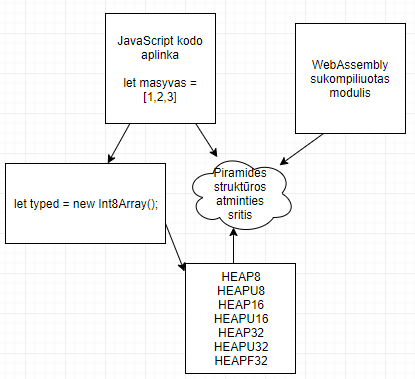
\includegraphics[scale=0.7]{wasm_heap.png}
  \end{center}
  \caption{Komunikacija naudojant piramidės atmintį}
  \label{fig:wasm_stack}
\end{figure}
Ši atminties sritis WebAssembly standarte yra tiesiog paprastas JavaScript objektas, kuris imituoja tradicinę C/C++ kalbų piramidės duomenų struktūrą, nes pastarosios pasiekti dėl saugumo priežasčių programuotojai galimybės neturi. 
Sudėtingų tipų perdavimą tarp JavaScript kodo ir WebAssembly modulio galima pavaizduoti \ref{fig:wasm_stack} paveikslėlyje nurodyta schema, kurioje matosi, jog komunikacija tarp aplinkų vyksta netiesiogiai, žiūrint į bendrą atminties sritį.

Svarbu paminėti, jog negalime į piramidę tiesiogiai patalpinti apibrėžto JavaScript masyvo, turime jį paversti į tipizuotą masyvo tipą, atitinkantį konkretaus tipo piramidę, nes vieno tipo piramidėje negalima laikyti skirtingo tipo duomenų — kitu atveju bus gaunami netikėti ir nesąmoningi rezultatai. 

Taigi, turėdami sukompiliuotą modulį ir jį iškviečiantį sugeneruotą surišantįjį JavaScript kodą, galime bandyti iškviesti aprašytą C rikiavimo funkciją iš naršyklės. Šiam tikslui naudojame integruotas WebAssembly standarto realizacijos \lstinline[columns=fixed]{Module.ccall() ir Module.cwrap()} funkcijas, leidžiančias perduoti parametrus į WebAssembly modulį ir grąžinti rezultatą į JavaScript aplinką atgal. Šiame pavyzdyje naudojame \lstinline[columns=fixed]{wasm—arrays.js} atviro kodo biblioteką, patalpintą GitHub saugykloje, kuri suteikia papildomą ccall ir cwrap funkcijų abstrakcijos lygmenį, skirtą patogesniam naudojimui. Taigi, naršyklės kode galime iškviesti mūsų rikiavimo funkciją perduodami skaičių masyvą:

\begin{center}
\begin{small}
\begin{verbatim}
        const res = ccallArrays(
          "bubbleSort",
          "array",
          ["array"],
          [[2, 1, 13, 4, 50]],
          { heapIn: "HEAP8", heapOut: "HEAP8", returnArraySize: 5 }
        );
        console.log(res);
\end{verbatim}
\end{small}
\end{center}

Pirmuoju parametru nurodome kviečiamą funkciją, antrasis parametras apibrėžia iš kviečiamos funkcijos grįžtantijį tipą, trečias ir ketvirtas — perduodamų parametrų tipus ir reikšmes, penktasis parametras — perduodamas objektas — apibrėžia jog naudosime WebAssembly HEAP8 (baito dydžio) sveikųjų skaičių piramidės atminties sritį. Įvykdžius \lstinline[columns=fixed]{ccallArrays} funkciją rezultato kintamasis \lstinline[columns=fixed]{res} gauna \lstinline[columns=fixed]{int8_t} tipo rodyklę, būtent tokio tipo, kokį apibrėžėme C funkcijoje. Ši rodyklė rodo į surikiuoto masyvo pradžios atminties sritį, todėl JavaScript kode galime pasiekti pakeistąjį masyvą. Našyklės konsolėje stebimas paveikslėjyje matomas kvietimo rezultatas.

\begin{figure}[h!]
  \begin{center}
  
\includegraphics[scale=0.7]{sorted_array.png}
  \end{center}
  \caption{Rezultatas naršyklės konsolės lange}
  \label{fig:sorted_array}
\end{figure}

Tagi, šiame pavyzdyje sugebėjome realizuoti logikos algoritmą C programavimo kalba, jį sukompiliuoti į WebAssembly modulį ir iškviesti JavaScript kode. Ši situacija parodo, jog WebAssembly standarto moduliarumo savybė leidžia skaičiavimams jautrias logikos sritis perkelti iš JavaScript kodo į WebAssembly modulius. Būtent todėl WebAssembly standartas ne pakeičia, o papildo JavaScript veikimą ten, kur pokytis atrodo racionalus ir reikalingas.

\subsubsection{Realaus pasaulio scenarijai}

Aprašytasis pavyzdys tik vaizdžiai parodo, kaip galima WebAssembly integruoti į egzistuojančią interneto sistemą pagerinant greitaveikos rodiklius. Taikant šį principą rinkoje galima paspartinti jau egzistuojančius sprendimus.

Vienas tokių atvejų galėtų būti ReactJS biblioteka, skirta kurti klientiniam interneto kodui. Esminis šios bibliotekos suderinimo (angl. — Reconciliation) algoritmas, skirtas efektyviai perpiešti DOM medį ir pastebėti, kurie šio medžio lapai pakeitė būseną, galėtų būti pakeistas WebAssembly realizacijos kodu išlaikant tokį patį programinį kontraktą React bibliotekos naudojams (angl. — API). Tokiu atveju vienintelis pokytis, kurį pajustų naudotojai — išaugusi bibliotekos veikimo sparta .

Kitas pavyzdys, kuris rinkoje jau implementuotas — kompanijos eBay programuotojų komandos sukurta internetinė brūkšninio kodo nuskaitymo programa, skirta eBay aukciono pardavėjams įkelti savo parduodamas prekes. Šis įrankis eBay programuotojų buvo sukurtas C++ kalba ir sėkmingai veikė iOS ir Android mobiliose aplinkose. Atsiradus WebAssembly technologijos realizacijai interneto naršyklėse, eBay programuotojai egzistuojančią kodo bazę sukompiliavo į .wasm modulį, rezultatas buvo stebinantis — lyginant su anksčiau veikusiu JavaScript brūkšninio kodo nuskaitymo įrankiu, kuris veikdavo vieno kadro per sekundę režimu, WebAssembly realizacija leido pasiekti 50 kartų didesnę greitaveiką.

\subsection{Naujo karkaso kūrimas WebAssembly pagrindu}
Vienas didžiausių standarto privalumų, kuro įtaką žiniatinkliui galima laikyti revoliucine, yra tai, jog WebAssembly mašininio kodo formatas skirtas būti kompiliuojamu iš skirtingų programavimo kalbų. Tai reiškia, jog JavaScript kalbos monopolis kuriant klientines interneto programas baigėsi. Anksčiau kuriant klientinę žiniatinklio sistemos dalį buvo būtina turėti plačias JavaScript kalbos ir ja parašytų karkasų ir bibliotekų, tokių kaip React, Angular, Vue žinias. Neteisinga teigti, jog JavaScript žinių nuo šiol nebereiks, tačiau žiniatinklyje vis daugiau vietos atsiras ir kitoms programavimo kalboms, kurias buvo įprasta matyti programuojant serverinę sistemos dalį.

Šis WebAssembly pritaikymo pavyzdys yra daug platesnis nei anksčiau aprašytasis centrinės logikos realizacijos pakeitimo, nes apima visą klientinės programos logikos perkėlimą į WebAssembly mašininį kodą.

Naujo karkaso kūrimo galimybes ir iššūkius naudojant WebAssembly kodą galima suprasti įsigilinus į jau realizuotus pavyzdžius, kurie, nors vis dar ankstyvose stadijose, tačiau jau nusako kryptį, kurios bus laikomasi.

\subsubsection{Microsoft .NET Blazor karkasas}
Microsoft kompanijos kuriamas .NET Blazor produktas — vartotojo sąsajos kūrimo C \# programavimo kalba karkasas, leidžiantis .NET programos kodui būti vykdomam tiesiogiai naršyklėje. Ši savybė leidžia programuotojams pernaudoti serverio dalyje esantį .NET kodą kuriant klientines programas.
\subsubsubsection{Platformos koncepcinė architektūra}
C \# kalbos kodo vykdymui reikalinga .NET vykdomoji aplinka, todėl esminis Blazor karkaso funkcinis vienetas yra Microsoft Xamarin komandos kuriama ir palaikoma Mono .NET vykdomoji aplinka, skirta mobiliųjų programėlių ir žaidimų konsolinėms platformoms kūrimui naudojant .NET technologijas. Nuo šiol ši vykdomoji aplinka veikia ir interneto naršyklėse — pastaroji buvo sukompiliuota į WebAssembly modulį. Šis modulis su savimi turi ir nebenaudojamų resursų surinkimo konstruktą (angl. — Garbage Collection), leidžiantį programuotojui nesirūpinti rankiniu atminties valdymu programuojant. Aukšto lygio Blazor veikimo principas nurodytas \ref{fig:blazor_architecture} schemoje, kur matome, jog mono.wasm — tai į WebAssembly mašininio kodo formatą sukompiliuota .NET Mono vykdomoji aplinka.

\begin{figure}[h!]
  \begin{center}
  \includegraphics[scale=0.9]{blazor_veikimo_architektūra.png}
  \end{center}
  \caption{Blazor karkaso veikimas naršyklėje}
  \label{fig:blazor_architecture}
\end{figure}

Verta paminėti, jog, kaip ir praeitame skyriuje demonstruotame pavyzdyje, kur buvo naudojamas Emscripten pagalba sugeneruotas JavaScript kodas, reikalingas užkrauti WebAssembly moduliui, turime \verb|mono.js| ir \verb|blazor.js| skriptus, reikalingus vykdomosios \verb|mono.wasm| aplinkos užkrovimui. Šis .NET vykdomomios Mono aplinkos režimas yra interpretuojamasis, nes mūsų kurta programa \verb|Programa.dll| nėra sukompiliuota į WebAssembly mašininį formatą, o interpretuojama pačioje kliento naršyklėje \verb|mono.wasm| modulio. Mono aplinka palaiko ir išankstinį (angl. — Ahead of Time) programos vykdymo būdą, kai mūsų kurta programa sukompiliuoajama į WebAssembly modulį iš anksto. Kaip pirmame skyriuje minėta, nėra fundamentaliai aišku, kuris modelis geresnis, tačiau interpretuojamas modelis daug artimesnis programavimui internete, nes kodo pokyčiai atsispindi naršyklės lange beveik iš karto — sukompiliavus pakeistą programos vietą, o taikant išankstinį modelį kompiliavimo žingsnis užtrunka pastebimai ilgiau, tačiau pats veikimo greitis greitaveikai jautriose vietose būna didesnis.

\subsubsubsection{Razor sintaksė Blazor klientinių žiniatinklio programų kūrime}
Faktas, jog visa klientinė programos logika perkeliama vykdyti WebAssembly moduliuose, leidžia beveik išsisukti be JavaScript kodo rašymo jį pakeičiant .NET pasaulyje gerai žinomai Razor sintaksei, kuri sujungia HTML, CSS žymėjimo kalbas ir C \# sintaksę viename faile:

\begin{center}
\begin{small}
\begin{verbatim}
@page "/skaitliukas"
<p>Dabartinis skaicius: @currentCount</p>
<button onclick="@IncrementCount">Padidinti</button>
@functions {
    int currentCount = 0;
    void IncrementCount()
    {
        currentCount++;
    }
}
\end{verbatim}
\end{small}
\end{center}

Pateiktame pavyzdyje parodyta \verb|<Counter>| vartotojo sąsajos komponento logika, kurioje paspaudus mygtuką skaitliukas padidinamas vientu. Dažniausiai tokį kodą dinamiškai vykdo JavaScript variklis, tačiau, kaip matome iš pavyzdžio, viskas rašoma naudojant tik HTML ir C \#, šiame pavyzdyje nedaroma jokių HTTP užklausų į nutolusį serverį. Direktyva \verb|@page| nurodo maršrutą, kuriuo bus pasiekamas komponentas.

\subsubsubsection{Blazor karkaso iššūkiai}
Kuriant serverio pusės logiką ASP.NET technologine platforma nebuvo itin aktuali surinkimo tekstų (angl. — .NET assemblies) užimama disko vieta serveryje — 2 MB ar 50 MB disko vietos užimantis kodas didelio skirtumo nedarydavo, tačiau naršyklės vykdyme šis aspektas yra kritinis, todėl net pritaikius Mono vykdomosios aplinkos ir programos kešavimo mechanizmą, yra itin svarbu, jog pirmasis puslapio užkrovimas, kurio metu parsiunčiama vykdomoji aplinka ir programinis kodas, būtų greitas. Technologijos kūrėjai pripažįsta, kad Blazor programa nesugebės pasiekti tokio suspaudimo lygio, kokį sugeba išgauti ReactJS biblioteka, tačiau pritaikius kelis optimizavimo metodus pasiekiamas rezultatas, leidžiantis galutiniam vartotojui sklandžiai naudotis klientine programa. Keli iš tų metodų yra:
\begin{itemize}
    \item HTPP užklausų atsakymų suspaudimas
    \item Kompiliavimo metu .NET IL surišiklis (angl. — Intermediate Language linker) statiškai skenuoja visą kodą ir pašalina tas dalis, kurios bus nenaudojamos kodo vykdymo metu
    \item .NET vykdomoji aplinka ir programos surinkimo failai kešuojami naršyklėje, kad nereiktų daryti nereikalingų užklausų į nutolusį serverį
\end{itemize}

\sectionnonum{Rez ultatai ir išvados}
Rezultatų ir išvadų dalyje turi būti aiškiai išdėstomi pagrindiniai darbo
rezultatai (kažkas išanalizuota, kažkas sukurta, kažkas įdiegta) ir pateikiamos
išvados (daromi nagrinėtų problemų sprendimo metodų palyginimai, teikiamos
rekomendacijos, akcentuojamos naujovės).


%% PAKEISTAS PAVADINIMAS Į 'Šaltiniai'
\addcontentsline{toc}{section}{Šaltiniai} 
\printbibliography[heading=bibintoc, title=Šaltiniai]  % Šaltinių sąraše nurodoma panaudota
\begin{thebibliography}{99}

\bibitem[LCW17]{LCW17} 
Lin Clark: A cartoon intro to WebAssembly, Žiūrėta[2019—06—07].  Prieiga internetu: \url{https://hacks.mozilla.org/2017/02/a—cartoon—intro—to—webassembly/}


\end{thebibliography}
% literatūra, kitokie šaltiniai. Abėcėlės tvarka išdėstomi darbe panaudotų
% (cituotų, perfrazuotų ar bent paminėtų) mokslo leidinių, kitokių publikacijų
% bibliografiniai aprašai.  Šaltinių sąrašas spausdinamas iš naujo puslapio.
% Aprašai pateikiami netransliteruoti. Šaltinių sąraše negali būti tokių
% šaltinių, kurie nebuvo paminėti tekste.

% \sectionnonum{Sąvokų apibrėžimai}
\sectionnonum{Santrumpos}
Sąvokų apibrėžimai ir santrumpų sąrašas sudaromas tada, kai darbo tekste
vartojami specialūs paaiškinimo reikalaujantys terminai ir rečiau sutinkamos
santrumpos.

\appendix  % Priedai
% Prieduose gali būti pateikiama pagalbinė, ypač darbo autoriaus savarankiškai
% parengta, medžiaga. Savarankiški priedai gali būti pateikiami ir
% kompaktiniame diske. Priedai taip pat numeruojami ir vadinami. Darbo tekstas
% su priedais susiejamas nuorodomis.

\section{Neuroninio tinklo struktūra}
\begin{figure}[H]
    \centering
    \includegraphics[scale=0.5]{img/MLP}
    \caption{Paveikslėlio pavyzdys}
    \label{img:mlp}
\end{figure}


\section{Eksperimentinio palyginimo rezultatai}
% tablesgenerator.com — converts calculators (e.g. excel) tables to LaTeX
\begin{table}[H]\footnotesize
  \centering
  \caption{Lentelės pavyzdys}
  {\begin{tabular}{|l|c|c|} \hline
    Algoritmas & $\bar{x}$ & $\sigma^{2}$ \\
    \hline
    Algoritmas A  & 1.6335    & 0.5584       \\
    Algoritmas B  & 1.7395    & 0.5647       \\
    \hline
  \end{tabular}}
  \label{tab:table example}
\end{table}

\end{document}
